For a quantum computer, multiple qubits are needed that are capable of interacting with each other. 
Thus, we need to make an array of the tweezers described in \cref{ch:tweezer}, spaced from each other in the order of micrometers. 
This can be done by sending different laser beams to the objective, all under slightly different angles. 

Experimentally, this could be realized using an \ac{AOD}: a device that diffracts light off of a sound wave in a crystal, where the degree of diffraction is controlled by a \ac{RF} signal. 
By using 2 AODs in an orthogonal configuration, each supplied by a superposition of RF signals, 2D Arrays have been succesfully realized \cite{Manuel2016}. 
This principle is sketched in \cref{fig:CrossAOD}.

\section{The Spatial Light Modulator}

One issue with this method is that there is little flexibility in varying the individual laser beam intensities, because of the crossed configuration this is impossible. 
Therefore, as early as \cite{Bergamini2004} it was proposed that a different method could be used to make tweezer arrays, which is to use a \ac{SLM}. 
This is effectively a mirror that can imprint a \ac{CGH} onto the impinging laser beam, such that in the focal plane of a lens arbitrary intensity patterns can be made. This technique has the advantage that one can flexibly control the potentials of each invididual tweezer, improving uniformity. 
In principle, it is even possible to make 3D arrays of tweezers \cite{DiLeonardo2007,Barredo2016}.

\subsection{Working Principle}

The \ac{SLM} can manipulate properties of light like amplitude, phase and polarization.
The type of SLM used is the phase-only SLM, and as the name suggests it can only control the phase of the light field.
It does this by deploying a large array of pixels, where each individual pixel has a liquid crytal in it. 
The orientation of the crystal will change the refractive index because of the birefringence effect. 
The pixelated display is manufactured on a layer of silicon to address the voltage of each cell invididually.
A sketch of the SLM pixels is shown in \cref{fig:LCoS}. 
The possibilities of this type of SLM has been documented extensively within our group, for example by \cite{Dijk2012,Bijnen2013,Bijnen2015}. 
\begin{figure}
\centering
	\begin{subfigure}{.4\textwidth}
		\centering
		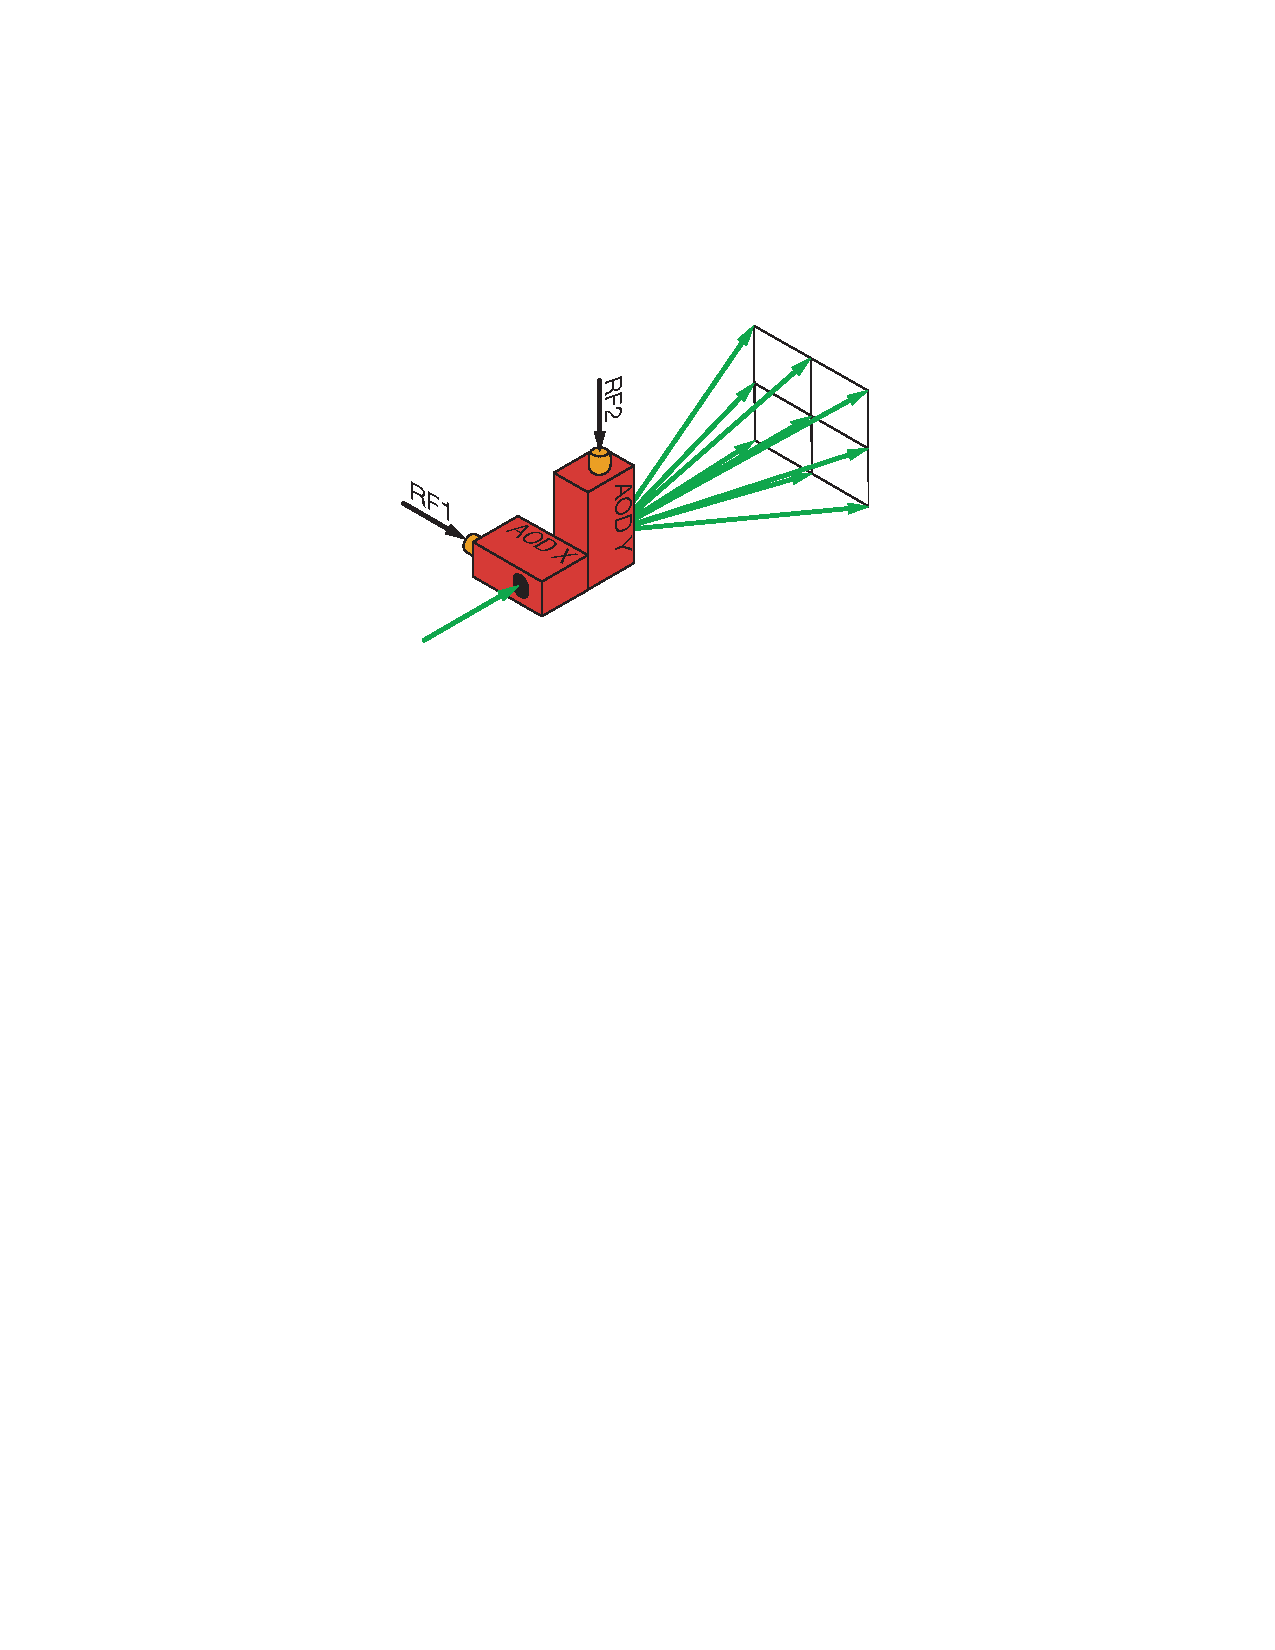
\includegraphics[height=3.8cm]{figures/crossAOD.pdf}
		\caption{}
		\label{fig:CrossAOD}
	\end{subfigure}
	\begin{subfigure}{.5\textwidth}
		\centering
		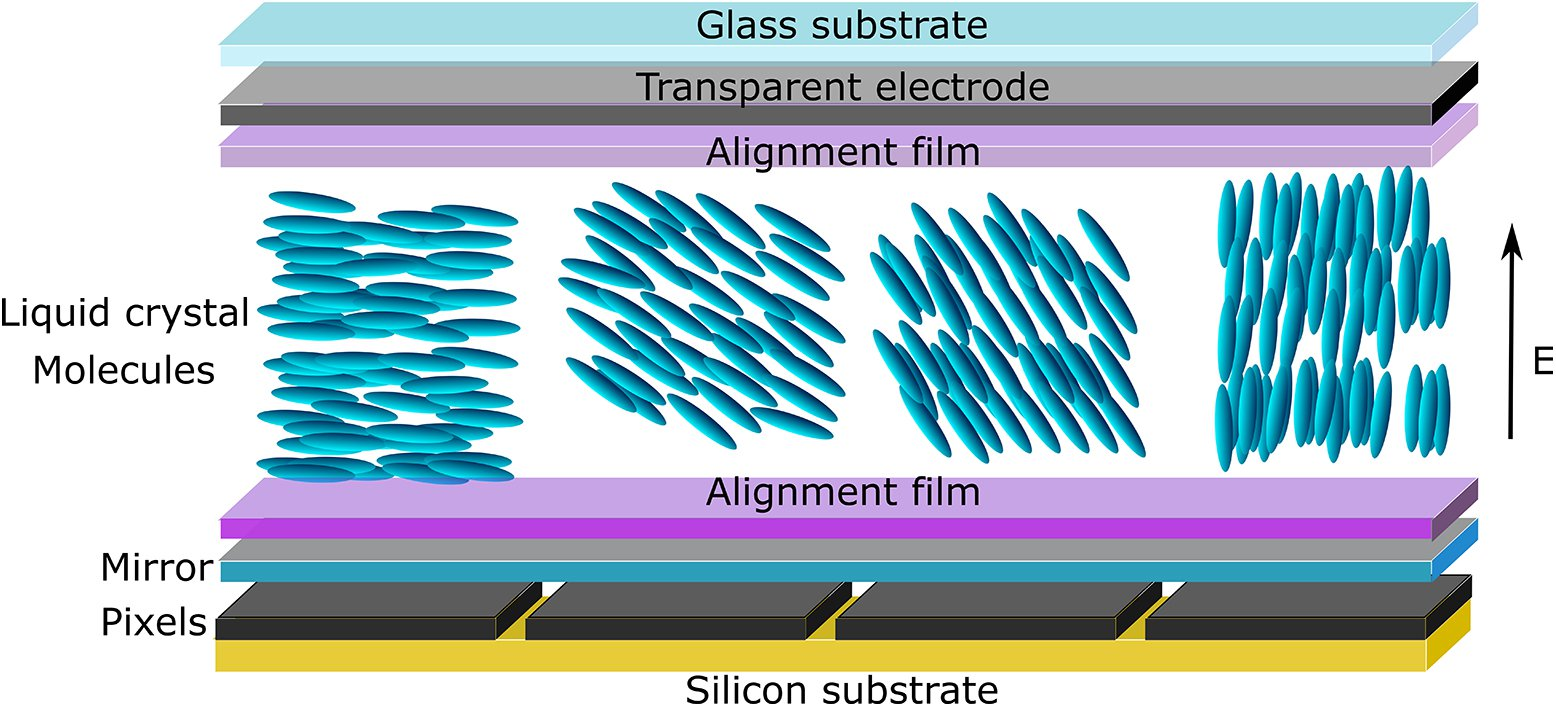
\includegraphics[height=3.8cm]{figures/LCoS.png}
		\caption{}
		\label{fig:LCoS}
	\end{subfigure}
	\caption{a) Two AODs in crossed configuration, used to make a 2D spot array. Figure from \cite{Cooper2018}. 
	b) The orientation of the liquid crystal cells changes as a function of the applied electric field $E$. 
	Figure from \cite{Guzman2017}.}
	\label{fig:GerschbergSaxton}
\end{figure}


\section{Phase Modulation}

In a phase only \ac{SLM}, each pixel can locally retard the field. 
As a result of diffraction, one can create arbitrary interference patterns in in the focal plane of the lens as shown by \cite{Bijnen2013}. 
The birefingence effect means the \ac{SLM} has two different refractive indices, somewhat confusingly called the ordinary and extraordinary refractive indeces respectively ($n_o$ and $n_e$). 
If the liquid crystal has a thickness $t$, the phase retardation will be $\phi_o = k t n_o$ and $\phi_e(V) = k t n_e(V)$ respectively, such that the phase retarder can be represented by the Jones matrix \cite{Guzman2017}

\begin{equation}\label{eq:JonesMatrix}
    M = e^{i \phi_0} 
    \begin{pmatrix}
        e^{i(\phi_e-\phi_o)} & 0\\
        0 & 1
    \end{pmatrix}
\end{equation}

Thus the phase retardance $\phi$ as a function of the applied voltage is \cite{Guzman2017}

\begin{equation}
    \phi(V) = k (n_e - n_0) t = \frac{2\pi}{\lambda} \Delta n t,
\end{equation}

where we absorbed the difference in refractive index in between the ordinary and extraordinary refractive indices in the paramter $\Delta n$.
This proces can be done separately for each pixel, leading to a phase retardance $
\phi(x',y')$ where $x',y'$ are the coordinates in the plane of the SLM. When a laser beam with intensity $|U_i|^2$ impinges on the SLM, it will pick up a phase. 
Thus its field can be described as $U_i e^{i\phi(x',y')}$ this is shown in \cref{fig:SLMgeometry}. 
The field will interfere with itself, until at infinity (or in the focal plane of a lens) the distribution evolves to $|U_f|^2$.
\cref{sec:PropagationDerivation,sec:GSW} delve deeper in how this quantitatively works. First we will note that the refractive index is not linear in the applied voltage, we thus need to calibrate the SLM first. 

\subsection{Calibration}

The retardiation is a result of the liquid crystal molecules rotating in their cells.
However, the retardation will not be linear as a function of the applied field $E$ and thus the voltage $V$. 
To linearize this, we need to calibrate the electro-optic response of the \ac{SLM}, which equates to measuring the retardation $\phi$ as a function of the applied voltage. 
This calibration serves two purposes:

\begin{enumerate}
    \itemsep=0pt
    
    \item Ensure the minimum to the maximum grey level corresponds to a $2\pi$ (one wave) phase retardation.
    
    \item Linearize the electro-optic response: that is the phase retardation as a function of grey level. 
\end{enumerate}


The light field will oscillate with frequencies in the THz regime thus measuring this phase shift directly is not practical. 
Instead, we use a method that measures the amount of power in the first diffraction order known as the diffractive method. 

There are a variety of methods to calibrate a phase-only \ac{SLM} \cite{Li2019}. 
We chose the diffractive calibration method, originally proposed by \cite{Zhang1994}.
We imprint a Ronchi grating onto the SLM, see \cref{fig:LUTCalibrationSetup}.
Consisting of alternating grey values $L_1$ and $L_2$.
This grating consists of $M$ periods $w$ in the horizontal direction and a vertical height $H$. 
Assuming amplitude modulation between different grey levels is negilible and the SLM only modulates phase, the electric field just after the SLM is propertional to the phase transmittance given by

\begin{equation}\label{eq:FieldAfterSLM}
    f(x,y) = \sum_{m=0}^{M-1} \left\{
    \operatorname{rect}\left(\frac{x-m w - w/4}{w/2}\right) + e^{i \phi(L)} \operatorname{rect}\left(\frac{x - m w - 3 w/4}{w/2}\right)
    \right\}
\end{equation}

According to Fourier optics, if we place a lens after the SLM, the field in the \textit{Fourier} plane of the lens is the Fourier transform of the field after the SLM, as derived in \cref{eq:2Dcase}.
The intensity is thus for $y=0$

\begin{equation}\label{eq:FourierIntensity}
    |F(p,0)|^2=
    \frac{M^2 w^2}{2}\operatorname{sinc}^2\left(\frac{M f_x w}{2}\right) \cdot
    \frac{1 + \cos{\left[\phi(L)+f_x w/2\right]}}{\cos^2(f_x w/4)}
\end{equation}

Such that the intensity in the first diffraction order is

\begin{equation}\label{eq:IntensityFirstOrder}
    I_1(\phi) =
    \frac{8M^2w^2}{\pi^2} \left( 
    1-\cos{\phi(L)}
    \right)
\end{equation}

\begin{figure}
	\begin{subfigure}{.54\linewidth}
		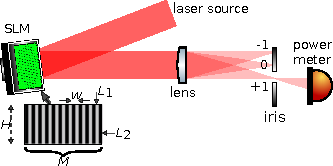
\includegraphics[height=4cm]{figures/LUTcalibrationSetup.pdf}
		\caption{}
		\label{fig:LUTCalibrationSetup}
	\end{subfigure}
	\hfill
	\begin{subfigure}{.44\linewidth}
		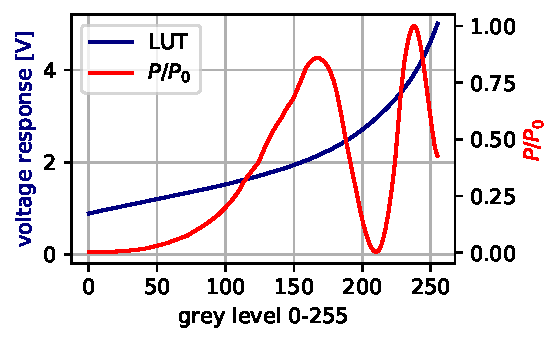
\includegraphics[height=4cm]{figures/lut_plot.pdf}
		\caption{}
		\label{fig:LUTcalibration}
	\end{subfigure}
	\caption{\textbf{a)} We put a Ronchi grating onto the SLM with grey values $L_1$ and $L_2$ We seperate the diffraction orders using a $f=400$ mm lens and block all orders other than the $+1$ order using an iris. 
	\textbf{b) }Normalized power in the first order as a (\textcolor{red}{red}) and the fitted voltage response (\textcolor{blue}{blue}) as a function of the applied grey level $L_1 \in (0-255)$.}
\end{figure}

Experimentally, we load a sequence of Ronchi gratings onto the SLM, looping $L_1$ from the minumum to the maximum grey value, while keeping $L_2$ consant. 
For our 8-bit SLM, this is 0-255. For each hologram, seperate the multiple diffraction orders using a longer focal length lens (such that the spacing between the various orders is sufficient) and an aperture and record the power in the first order using a power meter. 
The results are shown in \cref{fig:LUTcalibration}. Also shown is the result of fitting \cref{eq:IntensityFirstOrder}: the voltage response as a fuction of grey level. 
This is also called the gamma curve or \ac{LUT}.
The LUT is the 8-bit grey level to 10-bit voltage levels of the SLM, such that the electro-optic response is linear. 
As can be seen from \cref{fig:LUTcalibration}, the obtained LUT is rather non-linear.

The LUT calibration has to be performed because each individual SLM has a slightly different electro-optic response. 
Also, it is wavelength specific, which is why we performed it for the wavelenghts that we want to use for our optical tweezers. 

\section{Light Propagation}\label{sec:PropagationDerivation}

Finding the \ac{CGH} to be displayed onto the SLM is not trivial. We will now explain how this is done.
We consider the general case for 3D spot arrays, but will see that for 2D arrays a faster algorithm can be used. 
We consider an ensemble consisting of the SLM and a perfect lens with focal length $f$. We define two cartesian coordinate systems: the SLM plane by $\{x',y'\}$ and the focal plane of the lens by $\{x,y\}$. 
The situation is sketched in \cref{fig:SLMLens}

We adapt the following notation, the \ac{SLM} plane, with individual pixels indexed by $j$, such that the coordinates are $x'_j, y'_j,0$ ($z'=0)$ because by definition the pixels lie in this plane.
Next, we place a lens with focal length $f$ one focal length away from the SLM plane.
One focal plane further is the focal plane of this Fourier lens, which we call the Fourier plane. See \cref{fig:SLMgeometry}. 

\begin{figure}
    \centering
    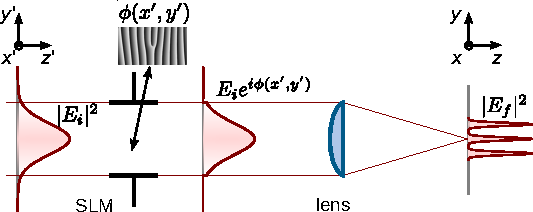
\includegraphics[width = 12cm]{figures/SLMfigure.pdf}
    \caption{Field with intensity distribution $|U_i|^2$ impinging on the SLM, which due to its finite size acts as an aperture.
    The lens makes the resulting image $|U_f|^2$ in its focal plane.
    Also shown: two cartesian coordinate systems in the SLM and focal plane. 
    Not to scale. 
    Adapted from \cite{Labuhn2016}.}
    \label{fig:SLMLens}
\end{figure}

When no phase is applied onto the SLM, the lens will focus all the light down to a diffraction-limited in the Fourier plane origin ($x=y=z=0$).
As result of traveling from the $j$th pixel to the $m$th trap, under paraxial approximation, the light picks up a phase along the way of 

\begin{equation}\label{eq:PropagationPhase}
    \Delta_j^m = \frac{2\pi z_m}{\lambdaup f^2}(x_j^2+y_j^2)+\frac{2\pi}{\lambdaup f}(x_j x_m +y_j y_m)
\end{equation}

This situation is sketched in \cref{fig:SLMgeometry}.
In the SLM plane, we assume uniform illumination of the SLM such that the amplitude is the same everywhere: $|E_i| = 1$.
This may look like an unrealistic assumption considering we use a gaussian input beam, but we will see in a moment that in fact the input beam does not matter for the pattern produced. 
The SLM imprints a phase $\phi(x',y') = \phi_j$, such that the complex amplitude in the SLM plane for pixel $j$ is

\begin{equation}
    U_j(x',y') = U_j e^{i \phi_j}
\end{equation}

The contribution for the $m$th trap can be found by summing over all pixels, also keeping track of a phase factor in what is known as the diffraction formula:

\begin{equation}\label{eq:DiffractionFormula}
    \nu_m = e^{i k \left(2 f + z_m\right)}
    \frac{d^2}{i \lambda f} \sum_{j=1}^N e^{i(\phi_j - \Delta_j^m)}
\end{equation}

Furthermore $d$ is the pixel pitch of the SLM. 
But we are not interested in the phase of each in every spot, but only in the intensity. 
We will thus emit the prefactors in \cref{eq:DiffractionFormula} and normalize over $N$ pixels

\begin{equation}\label{eq:Vm}
    V_m = \frac{1}{N} \sum_{j} e^{i(\phi_j - \Delta_j^m)}
\end{equation}

A subset of 3D spot arrays are to make 2D arrays. 
Setting $z=0$ in \cref{eq:Vm} yields 

\begin{equation}\label{eq:2Dcase}
    V_m = \frac{1}{N} \sum_j \exp{\left(i\phi_j\right)} \exp{\left(
    - i 2\pi \left[
    \frac{x_m}{\lambdaup f} x_j + \frac{y_m}{\lambdaup f} y_j
    \right]
    \right)}
\end{equation}

Which is the 2D \ac{DFT} of $e^{i\phi}$ evaluated at spatial frequencies $x_m/\lambdaup f$ and $y_m/\lambdaup f$ in $x$ and $y$ respectively \cite{DiLeonardo2007,Bijnen2015}. 
The DFT can be efficiently evaluated on a computer using a \ac{FFT}. We stress that the FFT can only be used for 2D arrays. 
In this work, we only use 2D arrays and could in principle use \cref{eq:2Dcase} to speed up calculation. 
We did not do this however, as we only have to calculate the \ac{CGH} once so we do not mind it taking some more time.
Making any arbitrary pattern in 2D, so not only spot arrays, is treated in detail in \cite{Bijnen2013}.  

This type of algorithm is very robust because as can be seen from \cref{eq:DiffractionFormula,eq:2Dcase}, the contribution for each spot $m$ really comes from all pixels $j$. 
This means that we do not need to know details about the exact input field used, which is really an advantage of this type of algorithm.

\section{Finding the Hologram}\label{sec:GSW}

\cref{eq:Vm} gives the amplitudes of an array of spots given an array of phases $\phi_j$, but we are interested in the reverse problem: what phase $\phi_j$ should we apply, such that we have the spot intensities $|V_m|^2$? 
Because the equations describing light progagation are time-symmetric, this phase will be the result of $N$ coherent light sources radiating with $w_m e^{i \theta_m}$, picking up a propagation phase described by \cref{eq:PropagationPhase}, leading to a complex amplitude in the \ac{SLM} plane of 

\begin{equation}\label{eq:InterferencePattern}
    U_j (x',y') = \sum_m w_m \exp{
    i\left(\Delta_j^m + \theta_j\right)
    }
\end{equation}

But requires doing phase as well as amplitude modulation, when the SLM can only do phase, which is to take the argument of \cref{eq:InterferencePattern}

\begin{equation}\label{eq:Argument}
    \phi_j = \text{arg}\left\{
     \sum_m w_m \exp{
    i\left(\Delta_j^m + \theta_j\right)
    }
    \right\}
\end{equation}

This problem was solved by \cite{Gerschberg1972} and extended to 3D spot arrays by \cite{DiLeonardo2007}. 
The idea is to make use of an algorithm that virtually propagates light back and forth between the SLM and focal planes.
For spot arrays, we are interested in the target intensities.
Summing all of them yields the real part of the interference pattern, or the diffraction efficiency $e$ as well as the uniformity $u$

\begin{equation}\label{eq:EfficiencyUniformity}
    e = \sum_m I_m = \sum_m |V_m|^2, 
    \quad 
    u = 1-\frac{\text{max}(I_m)-\text{min}(I_m)}{\text{max}(I_m)+\text{min}(I_m)}
\end{equation}

The algorithm should converge yielding a set $\{w_m, \phi_j\}$. 
]The iteration counter is $k$

\begin{itemize}
    \item Starting out with an initial guess $\phi_0$ using random phases for each pixel $\theta_j$ and uniform $w_m$, calculate $V_m$ according to \cref{eq:Vm}. 
    
    \item For In the focal plane, replace the calculated $V_m^k$ array by the target $V_m$ array and use this to calculate updated weight factors $w_m^k = w_m^{k-1} V_m^k / |V_m^k|$ find the new phase mask $\phi_j^k$ according to \cref{eq:InterferencePattern}.
\end{itemize}

This sequence is sketched in \cref{fig:GerschbergSaxton}. 
Starting with phase mask $\phi_j^k$ we use the diffraction equation \cref{eq:DiffractionFormula} to compute the complex amplitudes of the spot array $V_m^{k+1}$. 
From the amplitudes, we find new weight factors $w_m^k$ and pixel values $\theta_m^k$, which are used to compute the new phase mask using the interference equation \cref{eq:InterferencePattern}.
Then, the iteration counter $k$ is increased, the phase mask is updated and the procedure repeats. 

This type of algorithm typically converges after a couple tens of steps. The algorithm was implemented in Python by Ivo Knottnerus as part of his PhD research.
Because the SLM has some $\sim 2$ million pixels, converting to and from the SLM plane, so performing equations \cref{eq:Vm,eq:Argument} can be time consuming depending on the desired pattern.
Therefore, these computations are performed onto the GPU using the \textit{PyOpenCL} library. 

\begin{figure}
\centering
	\begin{subfigure}{.56\textwidth}
		\centering
		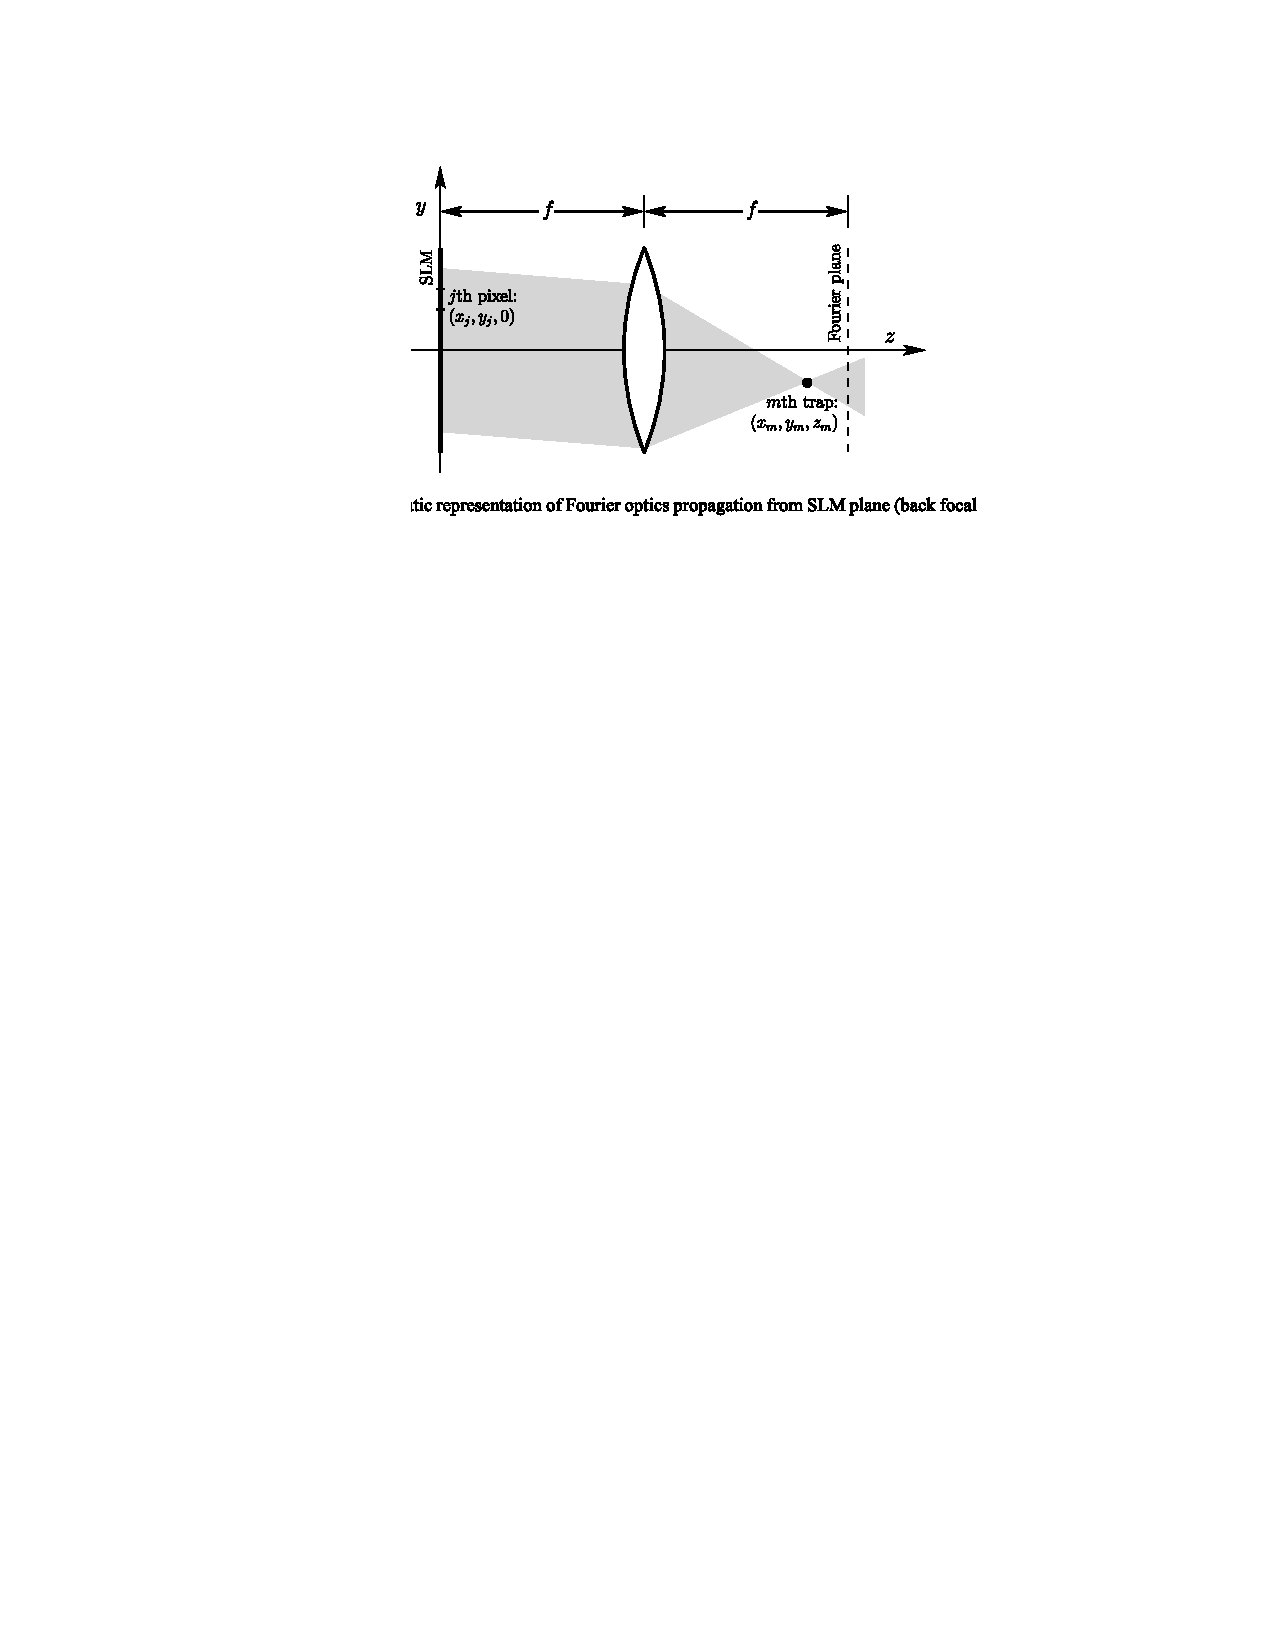
\includegraphics[height=5cm]{figures/SLMgeometry.pdf}
		\caption{}
		\label{fig:SLMgeometry}
	\end{subfigure}
	\begin{subfigure}{.43\textwidth}
		\centering
		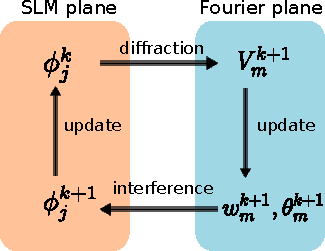
\includegraphics[height=5cm]{figures/WeightedGerschbergSaxton.pdf}
		\caption{}
		\label{fig:MOTconcept}
	\end{subfigure}
	\caption{\textbf{a)} SLM plane with phases $\phi_j(x,',y',z=0)$ for pixel $j$, as well as the focal plane or Fourier plane with trap coordinates for trap $m$ of $(x_m,y_m,z_m)$. 
	Figure from \cite{DiLeonardo2007}. 
	\textbf{b)} The \ac{GSW} algorithm visualized.
	The light field is virtually propagated between the SLM and focal planes using \cref{eq:Vm,eq:Argument}. 
	Each iteration, the weight factors $w_m$ and SLM phases $\theta_m$ are updated. }
	\label{fig:GerschbergSaxton}
\end{figure}


\section{Operating the SLM}

There are several practical considerations to be taken into account when operating the SLM. 
The most important ones will be discussed here. 

\subsection{Diffraction}\label{subsec:Diffraction}

Because the SLM has a lot of individual pixels with constant pitch $d$, the device acts effectively as a diffraction grating, so will be reflected in a variety of orders. 
It is well known from diffraction theory that in both $x$ and $y$ these diffraction angels $\theta_l$ of order $l$ occur at

\begin{equation}
    \theta_l = \arcsin\left(\sin\theta_i - l\frac{ \lambdaup}{d}\right)
\end{equation}

for incident angle $\theta_i$. 
The $l=0$ order contains the most power and is the only order that is used, the other orders are blocked using an aperture. 

But even if the higher diffraction orders are removed, there will always be a fraction of light that is not modulated. 
This is for example light coming from the space between the pixels as a result of the filling factor that is always lower than unity.
This undiffracted light is separated from the modulated light by imposing a linear phase on top of the pattern (tilt phase) which translate the pattern away from the undiffracted light.
Subsequently the undiffracted light is blocked in an intermediate focus point using an iris.
The type of linear phase used is shown in \cref{fig:Linear}.
Because the phase retardance is capped at $2\pi$, a sawtooth-like pattern emerges.
In reality, we use a period of just 8 pixels, but for the sake of visibililty we show a mask with a bigger period. 

\subsection{Finite Aperture Size}\label{subsec:ApertureSize}

In order to employ the maximum amount of degrees of freedom the SLM has to offer, and therefore the maximum drawing area in the focal plane of the Fourier lens, all of the pixels should be illuminated. 
However, because the incident beam is described by a gaussian, this will lead to power loss as a result of light not falling on the active pixel area. 
The ideal incident waist size is thus a compromise between power tranmission and degrees of freedom on the other.
    
We can estimate this power loss by shining a Gaussian beam $G(x,y)$ of width $w(z)$ and power $P_0$ onto a rectangular aperture of dimensions $(2S_x, 2S_y)$ where $S_{x,y}$ are the semi-widths of the aperture. 
The relative power transmission $P/P_0$ can be found by integrating the intensity of the beam \cref{eq:GaussianBeamIntensity} in cartesian coordinates over the aperture

\begin{equation}\label{eq:RectAperturePower}
    \frac{P}{P_0} =
    \iint G(x,y) dA=
    \text{erf}\left(\frac{\sqrt{2}S_x}{w(z)}\right) \text{erf}\left(\frac{\sqrt{2}S_y}{w(z)}\right)
\end{equation}

where erf($\cdot$) denotes the error function. 
The optimum incident beam size $w(z)$ is thus a compromize between drawing area and power efficiency. 
We have decied to use $w(z) = 4.8$ mm, which is about the size of the short axis $S_x = 4.9$ mm, such that we illuminate the entire \ac{SLM} and the power transmission as a result of the finite rectangular aperture is $\sim 95$\%.

\subsection{Demagnification}

The $w = 4.8$ mm beam needs to be adapted to the $R = 2$ mm radius of the microscope objective, in order to not lose almost all of the power. 
As discussed in \cref{ch:tweezer}, we use a 2 mm waist at the microscope objective, so the magnification should be $M = 2.0 / 4.8 \sim 0.42$. 
We do this by applying a lens phase onto the SLM shown in \cref{fig:Lens}. 
Finally, \cref{fig:Zernike} shows the Zernike correction pattern as found in \cref{ch:tweezer}.

\subsection{Optical Flatness}\label{subsec:Flatness}

Because of manufacturing imperfections, the SLM chip will not be perfectly flat on the scale of light wavelengths. 
This error is different for invididual SLM units.
The flatness of our chip was measured by manufacterer Meadowlark to have a RMS flatness of $\sim 0.18\lambdaup$.
The shape of the flatness was measured as well, so we can correct for the error by subtracting this phase pattern. 
The correction used is shown in \cref{fig:Flatness}.

\subsection{Total Phase Mask}

Because retardation of $2\pi$ has no effect, we can superimpose the various contributions to the phase pattern discussed in \cref{sec:GSW} and this section, and subsequently compute modulo $2\pi$ of the total phase. 
Here, we show the various phase masks that we have put onto the SLM:

\begin{figure}
	\begin{subfigure}{.18\linewidth}
		\centering
		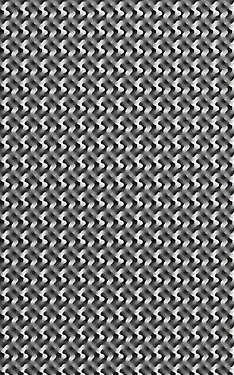
\includegraphics[height=4cm]{figures/SLMphase/array.jpg}
		\caption{}
		\label{fig:Array}
	\end{subfigure}
	%
	\begin{subfigure}{.18\linewidth}
		\centering
		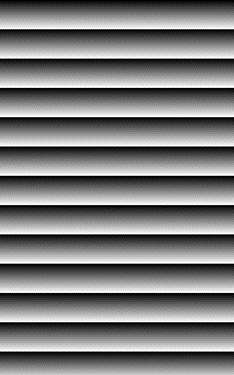
\includegraphics[height=4cm]{figures/SLMphase/linear.jpg}
		\caption{}
		\label{fig:Linear}
	\end{subfigure}
	%
	\begin{subfigure}{.18\linewidth}
		\centering
		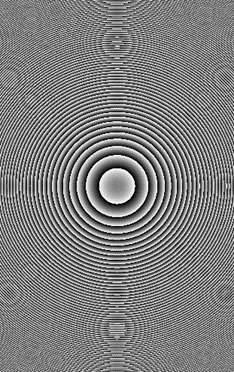
\includegraphics[height=4cm]{figures/SLMphase/lens.jpg}
		\caption{}
		\label{fig:Lens}
	\end{subfigure}	
	%
	\begin{subfigure}{.18\linewidth}
		\centering
		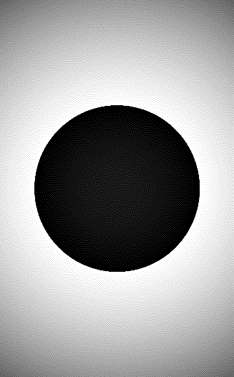
\includegraphics[height=4cm]{figures/SLMphase/flatness.jpg}
		\caption{}
		\label{fig:Flatness}
	\end{subfigure}
	%
	\begin{subfigure}{.18\linewidth}
		\centering
		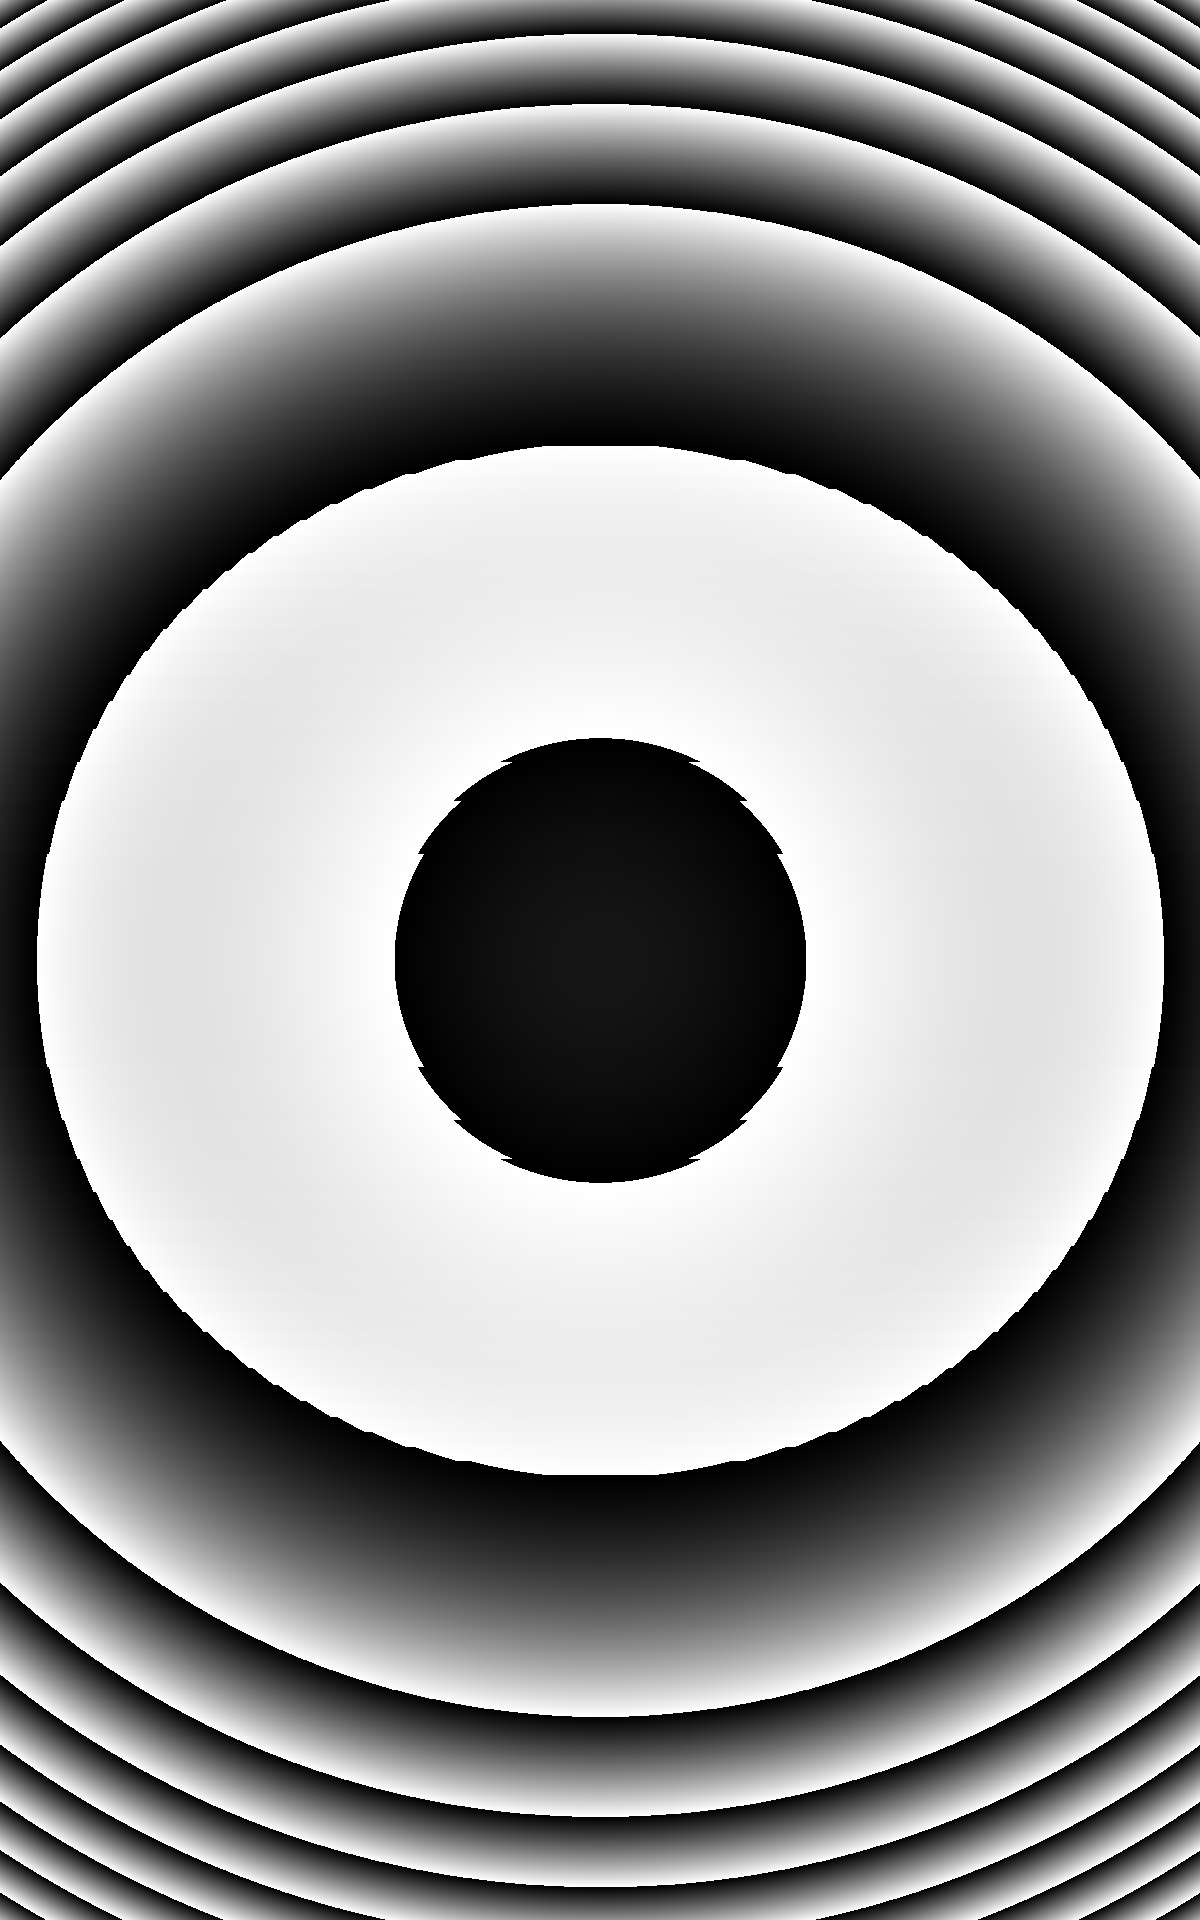
\includegraphics[height=4cm]{figures/SLMphase/zernike.jpg}
		\caption{}
		\label{fig:Zernike}
	\end{subfigure}
	%
	\begin{subfigure}{0.055\linewidth}
	    \centering
	    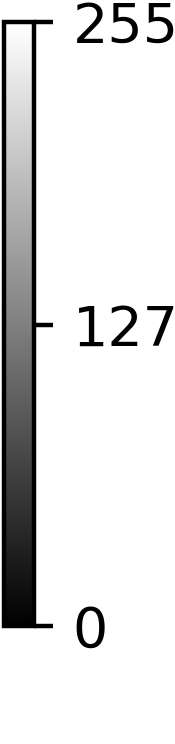
\includegraphics[height = 3.5cm]{figures/SLMphase/colorbar.jpg}
	\end{subfigure}
	%
	\caption{a) b)}
	\label{fig:SLMphase}
\end{figure}



\section{Arrays of tweezers}

Using holography and the SLM, we can make arbitrary arrays of spot using the algorithm discussed in \cref{sec:GSW}. 
We limited ourself to arrays of $n \times n \times 1$ pixels in the $x$, $y$ and $z$-directions respectively, where $n \in (1,2\ldots10)$. 
Phase masks were made using the algorithm implemented by Ivo Knottnerus running it for several hundred iterations, to get uniformities $>0.9999$ (In the \ac{GSW} algorithm, uniformities will get arbitrarily high for more iterations). 
In we show a result, where we plot the calculated diffraction pattern in the focal plane. The theoretical diffraction efficiency: the real part of the interference in the focal plane from the light propagation equation was found to be on the order of $e \sim 0.92$ (\cref{eq:EfficiencyUniformity}, irrespective of the amount of spots made, similar to the original publication of this algorithm \cite{DiLeonardo2007}.
In ... we show the theoretical diffraction result as found by the program, the computed hologram, as well as the measured pattern from the camera. 

\begin{mdframed}
    \subsection*{About the Units in the Fourier Plane}
    
    It is not nesessary necessary for the algorithm to take the exact optical setup into account.
    For the purposes of producing phase masks, we discard the telescope and treat the microscope objective as an ideal lens with focal length $f = 4$ mm, as also shown in \cref{fig:SLMgeometry}.
    In this case, smallest feature that can be produced in the Fourier plane is the diffraction-limited spot from the size of the SLM dimenions which can be considered a rectangualar aperture \cite{Bijnen2013,Bijnen2015}:
    
    \begin{equation}\label{eq:FocalUnit}
        \Delta x \times \Delta y = \frac{2\lambdaup f}{S_x} \times \frac{2 \lambdaup f}{S_y}
    \end{equation}
    
    \cref{eq:FocalUnit} are known as focal units and they are a natural unit to use in the Fourier plane.
    However, this will not fully apply to us, because we conjugate the short axis of the SLM to the aperture radius of the lens (objective), such that the extra pixels in the long axis of the SLM are effectively not used. 
    Therefore, we can set $S_x = S_y$ and the focal units will be the same in $x$ and $y$.
\end{mdframed}
    



\subsection{Spot Detection}

We make an arbitrarily sized array of optical tweezers. For detecting maxima locations, we could simply set pixels above a certain count threshold as a maxima. The disadvantage of this is that a noisy pixel could be detected as a spot, which would hinder analysis. 

To combat this, we first convolute the image with a Laplacian of Gaussian filter, which first smoothes the image to reduce noise. Subsequently it computes the 2D laplacian to detect edges. If this second derivative is above a certain threshold, we detect the edge as a spot. If the detected amount of spots is not the expected amount, we can easily tune the threshold. The camera image is cropped into regions of interest around the spots marked by the Laplacian of Gaussian filter. 

\subsection{Spot Fitting}

We fitted the tweezer arrays using the same Gaussian used in the previous chapter (\cref{eq:2DGaussian}, with for each spot, numbered $k$, 5 fit parameters: the amplitude ('trap depth') $U_0$, the peak center $(x_0, y_0)$ as well as the sigmas in both cartesian coordinates $\sigma_x$ and $\sigma_y$:

\begin{equation}\label{eq:2DGaussianNumberK}
    U_k(x,y) = U_{0,k}\exp{\left(\frac{-(x_k-x_{0,k})^2}{2\sigma_{x,k}^2}\right)}
    \exp{\left( \frac{-(y_k-y_{k,0})^2}{2\sigma_{k,y}^2} \right)}
\end{equation}

So in principle we allow non circular spots, but we extract the waist $w_k$ of each spot as $w_k = \sigma_{x,k} + \sigma_{y,k}$